\chapter{Evaluation}
All methods are evaluated on the held-out test split under a shared parsing and scoring protocol. Following common MOS-based IQA evaluation practice for LDCT quality assessment \cite{lee2025low}, we report absolute error, correlation, and prediction-coverage metrics. Let $\hat{y}_i$ denote the predicted MOS and $y_i$ the ground-truth MOS. The primary error metrics are
\begin{equation}
  \mathrm{MAE}=\frac{1}{N}\sum_{i=1}^{N}|\hat{y}_i-y_i|
\end{equation}
and
\begin{equation}
  \mathrm{RMSE}=\sqrt{\frac{1}{N}\sum_{i=1}^{N}(\hat{y}_i-y_i)^2}.
\end{equation}
MAE and RMSE quantify the absolute deviation of predicted scores from radiologist MOS targets. Because MOS prediction is also expected to preserve the relative ordering of image quality, we additionally report PLCC, SROCC, and KROCC as complementary correlation measures. PLCC captures linear agreement with the MOS scale, while SROCC and KROCC evaluate rank consistency. For generative models, prediction coverage is also reported because invalid or unparsable text completions can reduce the number of usable MOS estimates.

\section{Selected Models}
Model selection is based on SROCC, reflecting the goal of preserving the relative ordering of image quality. Table~\ref{tab:selected-results} compares four representative settings: the prompted base VLM, the SFT initialization checkpoint used for GRPO, the best pure SFT configuration, and the best SFT-initialized GRPO refinement.

\begin{table}[t]
  \centering
  \caption{Overall test-set MOS prediction comparison. Lower MAE/RMSE is better; higher correlation and coverage are better. Best configurations are selected by maximum SROCC.}
  \label{tab:selected-results}
  \scriptsize
  \setlength{\tabcolsep}{2pt}
  \resizebox{\linewidth}{!}{%
  \begin{tabular}{@{}lrrrrrr@{}}
    \toprule
    Model & MAE & RMSE & PLCC & SROCC & KROCC & Coverage \\
    \midrule
    Direct base VLM & 4.453 & 5.395 & 0.014 & -0.020 & -0.016 & 100.0\% \\
    SFT init. & \textbf{0.347} & \textbf{0.451} & 0.916 & 0.917 & 0.787 & 100.0\% \\
    Best SFT & 0.393 & 0.482 & \textbf{0.930} & \textbf{0.932} & \textbf{0.808} & 100.0\% \\
    Best SFT+GRPO & 0.666 & 0.796 & 0.897 & 0.907 & 0.788 & 100.0\% \\
    \bottomrule
  \end{tabular}
  }
\end{table}

The row denoted SFT init.\ is the standalone supervised adapter used as the starting point for GRPO. It is not the strongest SFT model by SROCC, but it provides the lowest MAE and RMSE. Best SFT is selected separately from the SFT ablation and gives the strongest overall correlation metrics. The best SFT-initialized GRPO run substantially improves over direct prompting and narrows the gap to supervised adaptation, but it does not surpass the SFT models.

\section{SFT Parameter Study}
The SFT ablation is organized around a reference configuration with two epochs, learning rate $2{\times}10^{-4}$, LoRA rank 16, and dropout 0.05. We then vary one factor at a time: epoch count, learning rate, LoRA rank, or dropout. LoRA rank $r$ is the dimensionality of the trainable low-rank adapter update; reducing $r$ lowers adapter capacity and the number of trainable parameters. All configurations produce valid MOS predictions for all 300 test samples. Table~\ref{tab:sft-study} shows that SFT is stable across the top configurations: the rank-8 adapter gives the strongest SROCC, the rank-32 adapter gives the strongest KROCC, and three epochs gives the strongest PLCC. In contrast, lowering the learning rate to $5{\times}10^{-5}$ or removing dropout reduces rank consistency. Thus, higher adapter capacity is not consistently beneficial, and the selected rank-8 model provides the best ordering performance under the SROCC selection criterion.

\begin{table}[t]
  \centering
  \caption{SFT ablation study around a rank-16 reference configuration. All runs have 100\% prediction coverage.}
  \label{tab:sft-study}
  \scriptsize
  \setlength{\tabcolsep}{2pt}
  \resizebox{\linewidth}{!}{%
  \begin{tabular}{@{}cccccrrrr@{}}
    \toprule
    Exp ID & Epochs & LR & $r$ & Dropout & MAE & PLCC & SROCC & KROCC \\
    \midrule
    A & 2 & $2{\times}10^{-4}$ & 16 & 0.05 & 0.384 & 0.930 & 0.931 & 0.804 \\
    B & 1 & $2{\times}10^{-4}$ & 16 & 0.05 & \textbf{0.360} & 0.919 & 0.922 & 0.794 \\
    C & 3 & $2{\times}10^{-4}$ & 16 & 0.05 & 0.368 & \textbf{0.933} & 0.932 & 0.807 \\
    D & 2 & $1{\times}10^{-4}$ & 16 & 0.05 & 0.374 & 0.931 & 0.932 & 0.804 \\
    E & 2 & $5{\times}10^{-5}$ & 16 & 0.05 & 0.416 & 0.922 & 0.923 & 0.792 \\
    F & 2 & $2{\times}10^{-4}$ & 8 & 0.05 & 0.393 & 0.930 & \textbf{0.932} & 0.808 \\
    G & 2 & $2{\times}10^{-4}$ & 32 & 0.05 & 0.367 & 0.929 & 0.930 & \textbf{0.809} \\
    H & 2 & $2{\times}10^{-4}$ & 16 & 0.00 & 0.376 & 0.926 & 0.926 & 0.802 \\
    I & 2 & $2{\times}10^{-4}$ & 16 & 0.10 & 0.376 & 0.928 & 0.929 & 0.804 \\
    \bottomrule
  \end{tabular}
  }
\end{table}

\section{GRPO Parameter Study}
The GRPO ablation evaluates the effect of initialization, learning rate, KL regularization, sampling temperature, candidate-group size, and completion length. As shown in Table~\ref{tab:grpo-study}, SFT initialization is important: runs initialized directly from the base VLM have weak correlations and lower coverage. Among SFT-initialized runs, increasing the learning rate to $2{\times}10^{-5}$ gives the strongest PLCC and SROCC while maintaining complete coverage. Shorter completions also improve rank consistency, achieving the strongest KROCC among the GRPO runs. In contrast, high sampling temperature and a smaller group of two completions sharply reduce coverage, indicating that reward-based MOS adaptation remains sensitive to generation validity.

\begin{table}[t]
  \centering
  \caption{GRPO ablation study over initialization, optimization, and generation settings.}
  \label{tab:grpo-study}
  \tiny
  \setlength{\tabcolsep}{1.4pt}
  \resizebox{\linewidth}{!}{%
  \begin{tabular}{@{}cccccccrrrrr@{}}
    \toprule
    Exp ID & Init. & LR & $\beta$ & Temp. & G & Len. & MAE & PLCC & SROCC & KROCC & Coverage \\
    \midrule
    A & SFT & $1{\times}10^{-5}$ & 0 & 0.7 & 4 & 32 & 0.690 & 0.854 & 0.883 & 0.763 & 99.3\% \\
    B & SFT & $2{\times}10^{-5}$ & 0 & 0.7 & 4 & 32 & 0.666 & \textbf{0.897} & \textbf{0.907} & 0.788 & 100.0\% \\
    C & SFT & $5{\times}10^{-6}$ & 0 & 0.7 & 4 & 32 & 0.654 & 0.859 & 0.883 & 0.764 & 100.0\% \\
    D & SFT & $1{\times}10^{-5}$ & 0.02 & 0.7 & 4 & 32 & \textbf{0.654} & 0.854 & 0.877 & 0.759 & 97.0\% \\
    E & SFT & $1{\times}10^{-5}$ & 0.05 & 0.7 & 4 & 32 & 0.662 & 0.857 & 0.877 & 0.756 & 100.0\% \\
    F & SFT & $1{\times}10^{-5}$ & 0 & 0.3 & 4 & 32 & 0.681 & 0.854 & 0.876 & 0.756 & 100.0\% \\
    G & SFT & $1{\times}10^{-5}$ & 0 & 1.0 & 4 & 32 & 0.795 & 0.762 & 0.814 & 0.705 & 55.3\% \\
    H & SFT & $1{\times}10^{-5}$ & 0 & 0.7 & 2 & 32 & 1.043 & 0.397 & 0.270 & 0.219 & 4.7\% \\
    I & SFT & $1{\times}10^{-5}$ & 0 & 0.7 & 4 & 16 & 0.658 & 0.874 & 0.902 & \textbf{0.789} & 100.0\% \\
    J & SFT & $1{\times}10^{-5}$ & 0 & 0.7 & 4 & 48 & 0.683 & 0.869 & 0.881 & 0.764 & 100.0\% \\
    K & Base & $1{\times}10^{-5}$ & 0 & 0.7 & 4 & 32 & 0.974 & 0.076 & 0.073 & 0.061 & 89.3\% \\
    L & Base & $5{\times}10^{-6}$ & 0 & 0.7 & 4 & 32 & 1.027 & -0.042 & -0.042 & -0.035 & 89.3\% \\
    \bottomrule
  \end{tabular}
  }
\end{table}

\begin{figure}[t]
  \centering
  
\includegraphics[width=\linewidth]{figures/sft_selected_scatter.png}
  \caption{Predicted versus ground-truth MOS for the selected SFT run. The dashed line denotes ideal agreement. Overall, 71.3\% of predictions fall within $\pm0.5$ MOS of the reference score.}
  \label{fig:sft-selected-scatter}
\end{figure}

\begin{figure}[t]
  \centering
  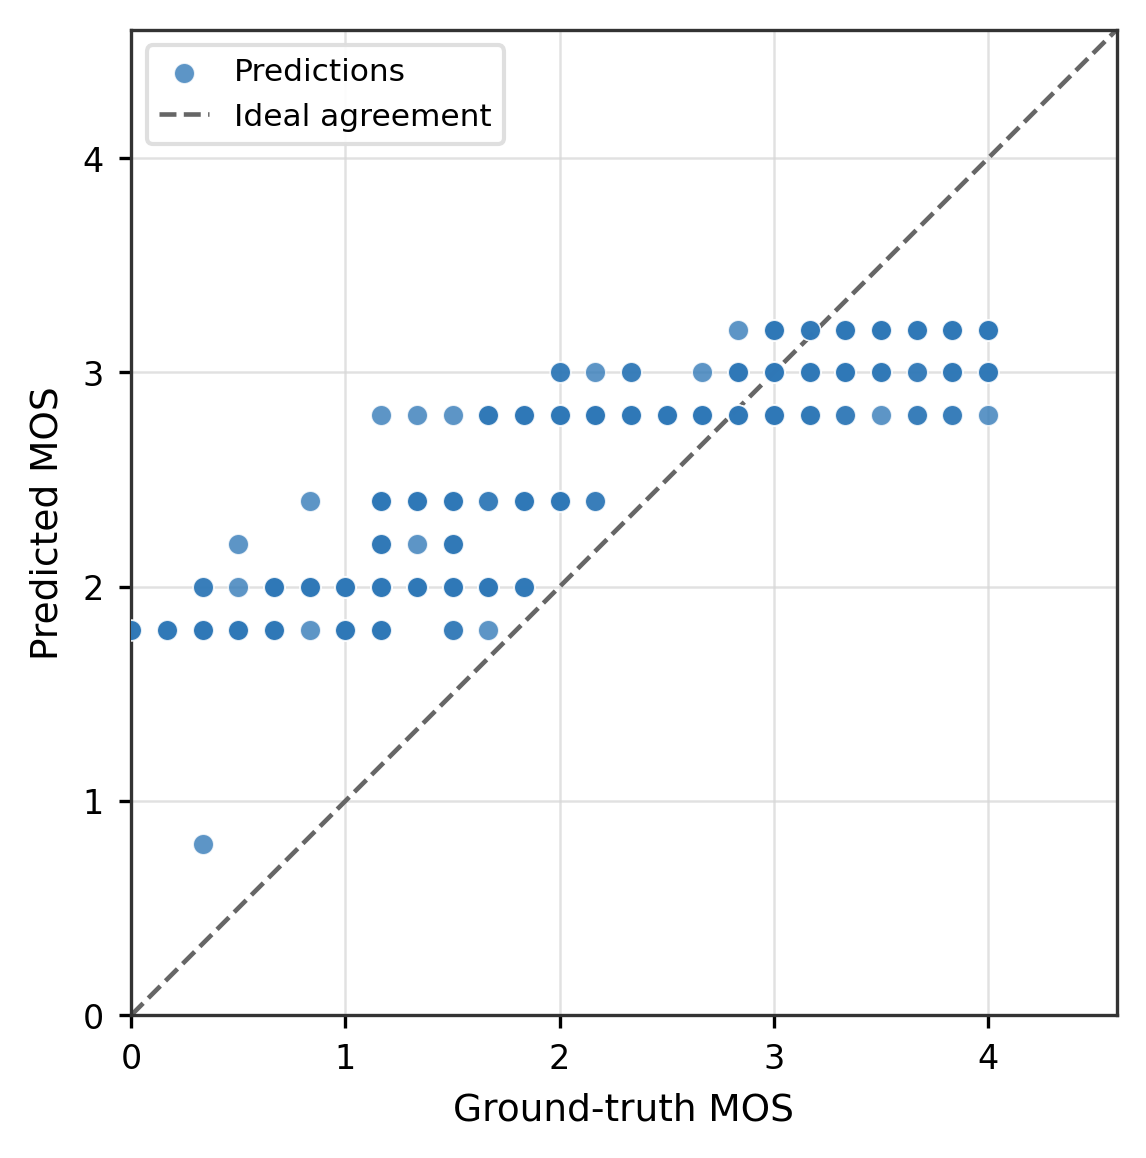
\includegraphics[width=\linewidth]{figures/grpo_selected_scatter.png}
  \caption{Predicted versus ground-truth MOS for the selected SFT-initialized GRPO run. The discrete prediction bands indicate remaining score-range compression after reward-based refinement. Overall, 43.3\% of predictions fall within $\pm0.5$ MOS of the reference score.}
  \label{fig:grpo-selected-scatter}
\end{figure}
